\documentclass[10pt,a4paper,twoside]{article}
\usepackage{latexsym}      % needed math symbols
\usepackage{hyperref}
\hypersetup{
 colorlinks=true,
 citecolor=blue,
 linkcolor=blue,
 urlcolor=blue,
 pdfpagemode=UseNone,
 pdfstartview=FitH}
\usepackage{graphicx}      % for importing eps figures
\usepackage{amsmath}       % for advanced math symbols
\usepackage[affil-sl]{authblk} 			% found in preprint bundle package, http://ctan.org/pkg/preprint
\usepackage[margin=2.5cm]{geometry} % paper and margin formats as set by SPP
\usepackage{subfig}

\parindent 0.5cm    % paragraphs indent
\topmargin=-2cm

% SPP details
\newcommand{\spp}{38\textsuperscript{th}}
\newcommand{\sppvenue}{Legazpi City, Albay}
\newcommand{\sppdate}{3--6 June 2020}


% title style
\newcommand*{\TitleFont}{\bfseries \Large }

% authblk style
\newcommand{\authorsep}{,\negmedspace}
\newcommand{\lastauthorsep}{}
\makeatletter
\renewcommand\AB@authnote[1]{{\textsuperscript{\normalfont#1}\ }}
\renewcommand\Authsep{}
\renewcommand\Authands{and }
\renewcommand\Authfont{\small {\bfseries}}
\renewcommand\Affilfont{\small	\itshape}
\setlength{\affilsep}{5pt}
\makeatother
\newcommand{\corremail}{\rm Corresponding author:~}

% remove date
\date{}

% for abstract style
\makeatletter
\newbox\abstract@box
\renewenvironment{abstract}
   {\global\setbox\abstract@box=\vbox\bgroup
     \hsize=\textwidth\linewidth=\textwidth
    \vspace{-2em}
		\small
		%\begin{center}
		{\hspace{1.2em}\bfseries \abstractname\vspace{.0em}\vspace{\z@} }%
		%\end{center}
    \quotation}
  {\endquotation\egroup}
\expandafter\def\expandafter\@maketitle\expandafter{\@maketitle
	\ifvoid\abstract@box\else\unvbox\abstract@box\if@twocolumn\vskip1.5em\fi\fi}
\makeatother
\providecommand{\keywords}[1]{\vspace{.5em}\noindent \mdseries{{Keywords:}} #1}
\providecommand{\DOI}[1]{\vspace{#1\baselineskip}}
\providecommand{\dateline}[1]{\vspace*{-1\baselineskip}\normalsize Submitted: #1\vspace*{-1.5\baselineskip}}

% for section formatting style
\makeatletter
\renewcommand\section{\@startsection
   {section}{1}{0pt}%
   {-\baselineskip}%
   {0.1\baselineskip}%
   {\normalfont\large\bfseries}}%
\renewcommand\subsection{\@startsection
   {subsection}{1}{0pt}%
   {-\baselineskip}%
   {0.1\baselineskip}%
   {\normalfont\bfseries}}%
\makeatother
\renewcommand\thesection{\arabic{section}}

% for the figure and tables, captions
\usepackage{booktabs}
\usepackage{dcolumn}
\newcolumntype{d}[1]{D{.}{.}{#1}}

\usepackage{caption}
\captionsetup[table]{position=above,font={rm,small}}
\captionsetup[figure]{font={rm,small}}

% for citations formatting style
\usepackage[numbers,square,sort&compress]{natbib}
\setlength\bibsep{1pt}

%%for first page styling 
\providecommand{\articlenum}[0]{}
\usepackage{fancyhdr}
\fancypagestyle{titlestyle}
{
\renewcommand{\headrulewidth}{0pt}
\renewcommand{\footrulewidth}{0.1pt}
\fancyhf[l]{}
\fancyhf[c]{ }
\fancyhf[r]{ }
\fancyfoot[l]{}
\fancyfoot[c]{\href{https://paperview.spp-online.org/proceedings/issue/archive}{Proceedings of the Samahang Pisika ng Pilipinas} \\ \href{https://paperview.spp-online.org/proceedings/issue/view/SPP-2020}{\spp\,Samahang Pisika ng Pilipinas Physics Conference}\\ \sppvenue, \sppdate \\ \articlenum 1}
\fancyfoot[r]{}
}

% styling for the second page onwards
\renewcommand{\headrulewidth}{0pt}
\renewcommand{\footrulewidth}{0.1pt}
\fancyhf[l]{}
\fancyhf[r]{}
\fancyhf[c]{}
\fancyfoot[l]{}
\fancyfoot[c]{\href{https://paperview.spp-online.org/proceedings/issue/archive}{Proceedings of the Samahang Pisika ng Pilipinas}  \\ \href{https://paperview.spp-online.org/proceedings/issue/view/SPP-2020}{\spp\,Samahang Pisika ng Pilipinas Physics Conference}\\ \sppvenue, \sppdate \\ \articlenum \thepage}
\fancyfoot[r]{}
\pagestyle{fancy}

% other packages and macros
\usepackage{bm}
\renewcommand{\vec}[1]{\text{\bfseries #1}}


%  Editorial staff will uncomment the next line
% \providecommand{\artnum}[0]{XX-XX}
% \renewcommand{\articlenum}[0]{SPP-\the\year-\artnum-}

\begin{document}

\title{\TitleFont Compressive Sensing: Applications from 1-D to $N$-D}

\author[*\negthickspace]{Kenneth V.~Domingo}
\author[ ]{Maricor N.~Soriano
\lastauthorsep}
\affil[ ]{National Institute of Physics, University of the Philippines, Diliman, Quezon City, Philippines}
\affil[*]{\corremail{kdomingo@nip.upd.edu.ph} }


\begin{abstract}
\noindent
Modern signal acquisition technologies are made possible by the Nyquist-Shannon sampling theorem (NST). However, this paradigm is extremely wasteful as the signal is compressed before storing it by systematically discarding the imperceptible information. Compressive sensing (CS) aims to directly sense the information that would otherwise survive this compression stage. Current literature focus exclusively on either audio or image signals, as well as quantifying their reconstruction quality with ambiguous metrics. In this paper, we compressively sample signals of arbitrary dimensions such as those consisting of combinations of audio and images, as well as quantify the reconstruction quality using metrics that are perceptually intuitive.

\keywords{compressive sensing, sub-Nyquist sampling, signal processing}

\end{abstract}

\maketitle
\thispagestyle{titlestyle}

\section{Introduction}\label{sec:intro}

\begin{figure}[tb]
\centering
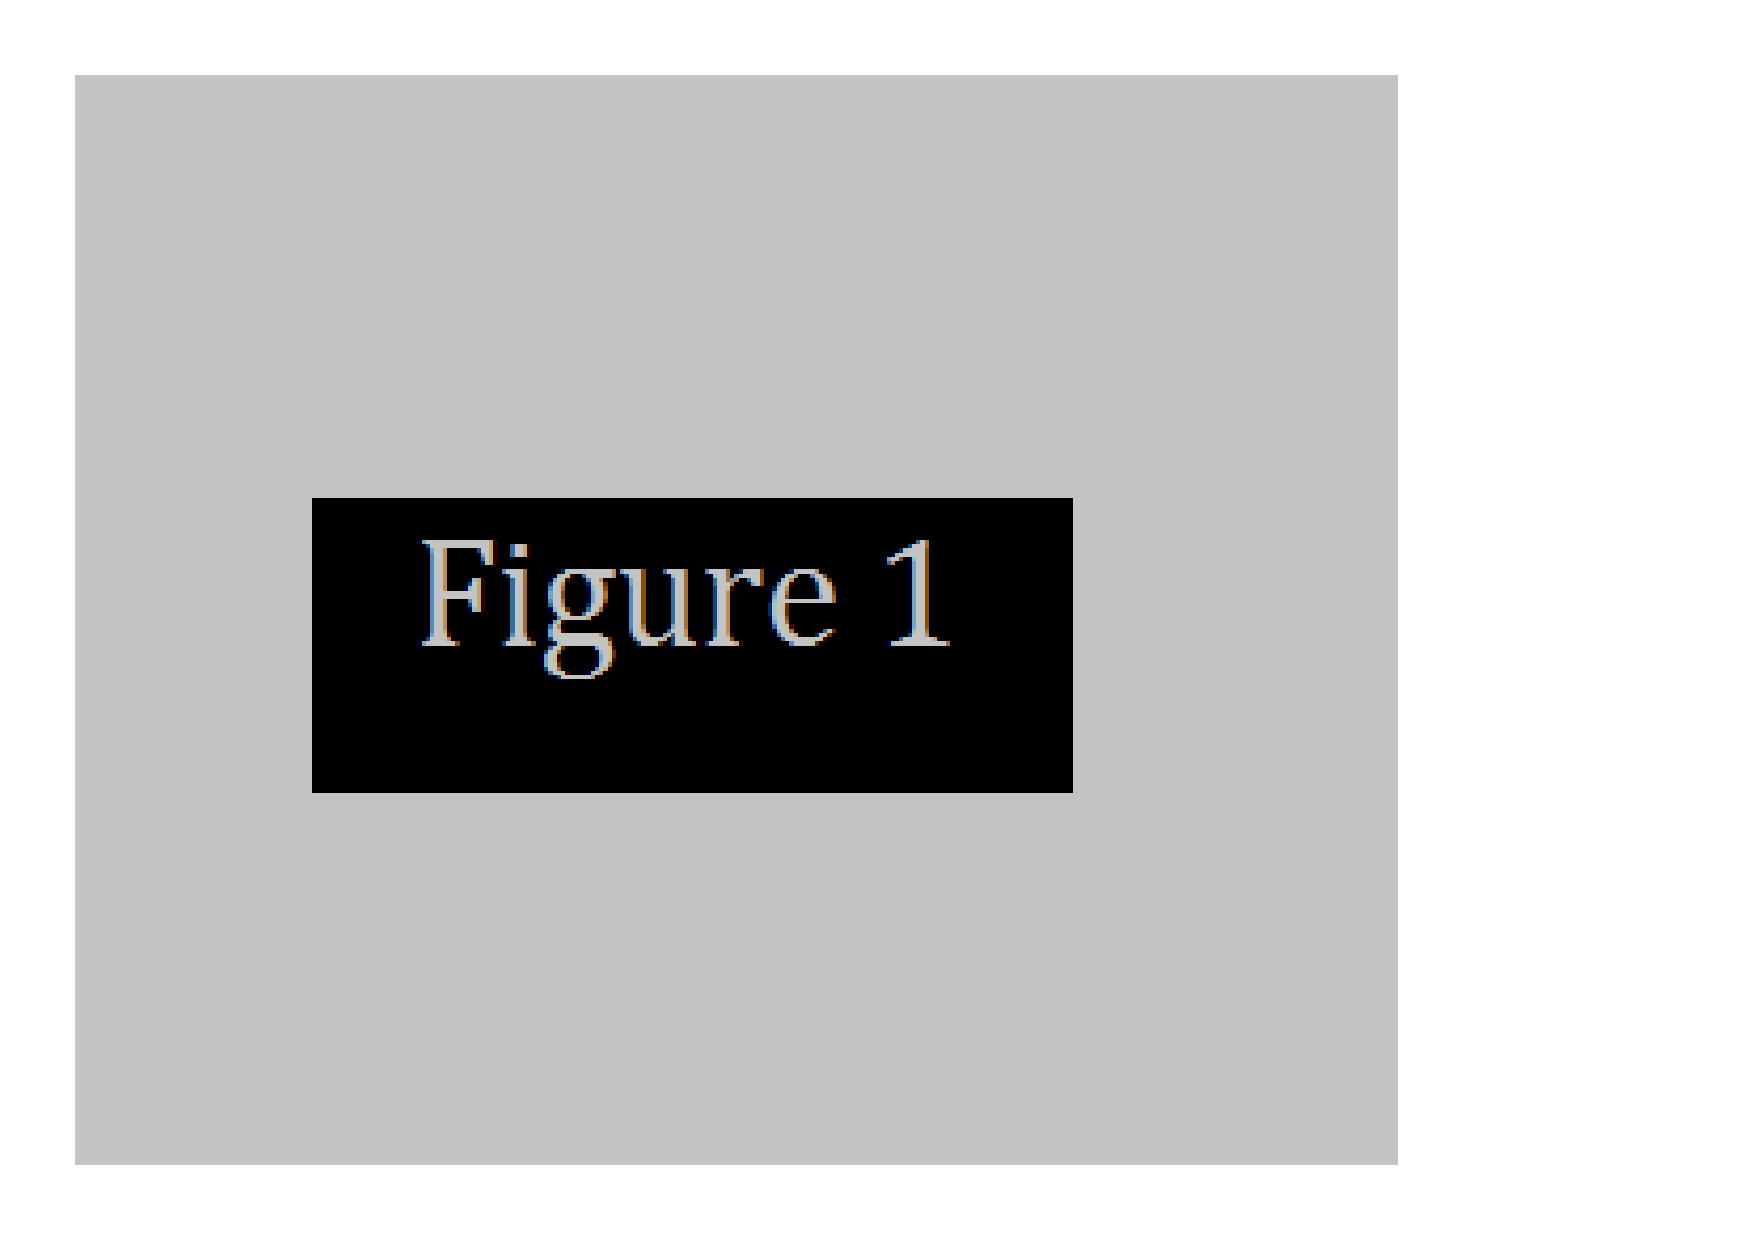
\includegraphics[width=0.3\linewidth]{figure1.pdf}
\caption{This is an example of a single column-wide figure. Figure captions are preferably self-contained and in vector format (versus raster format).}
\label{fig:plot1}
\end{figure}

\begin{figure}[tbp]
  \centering
  \subfloat[Optional subcaption of this subfigure.]{\makebox[0.4\textwidth]{{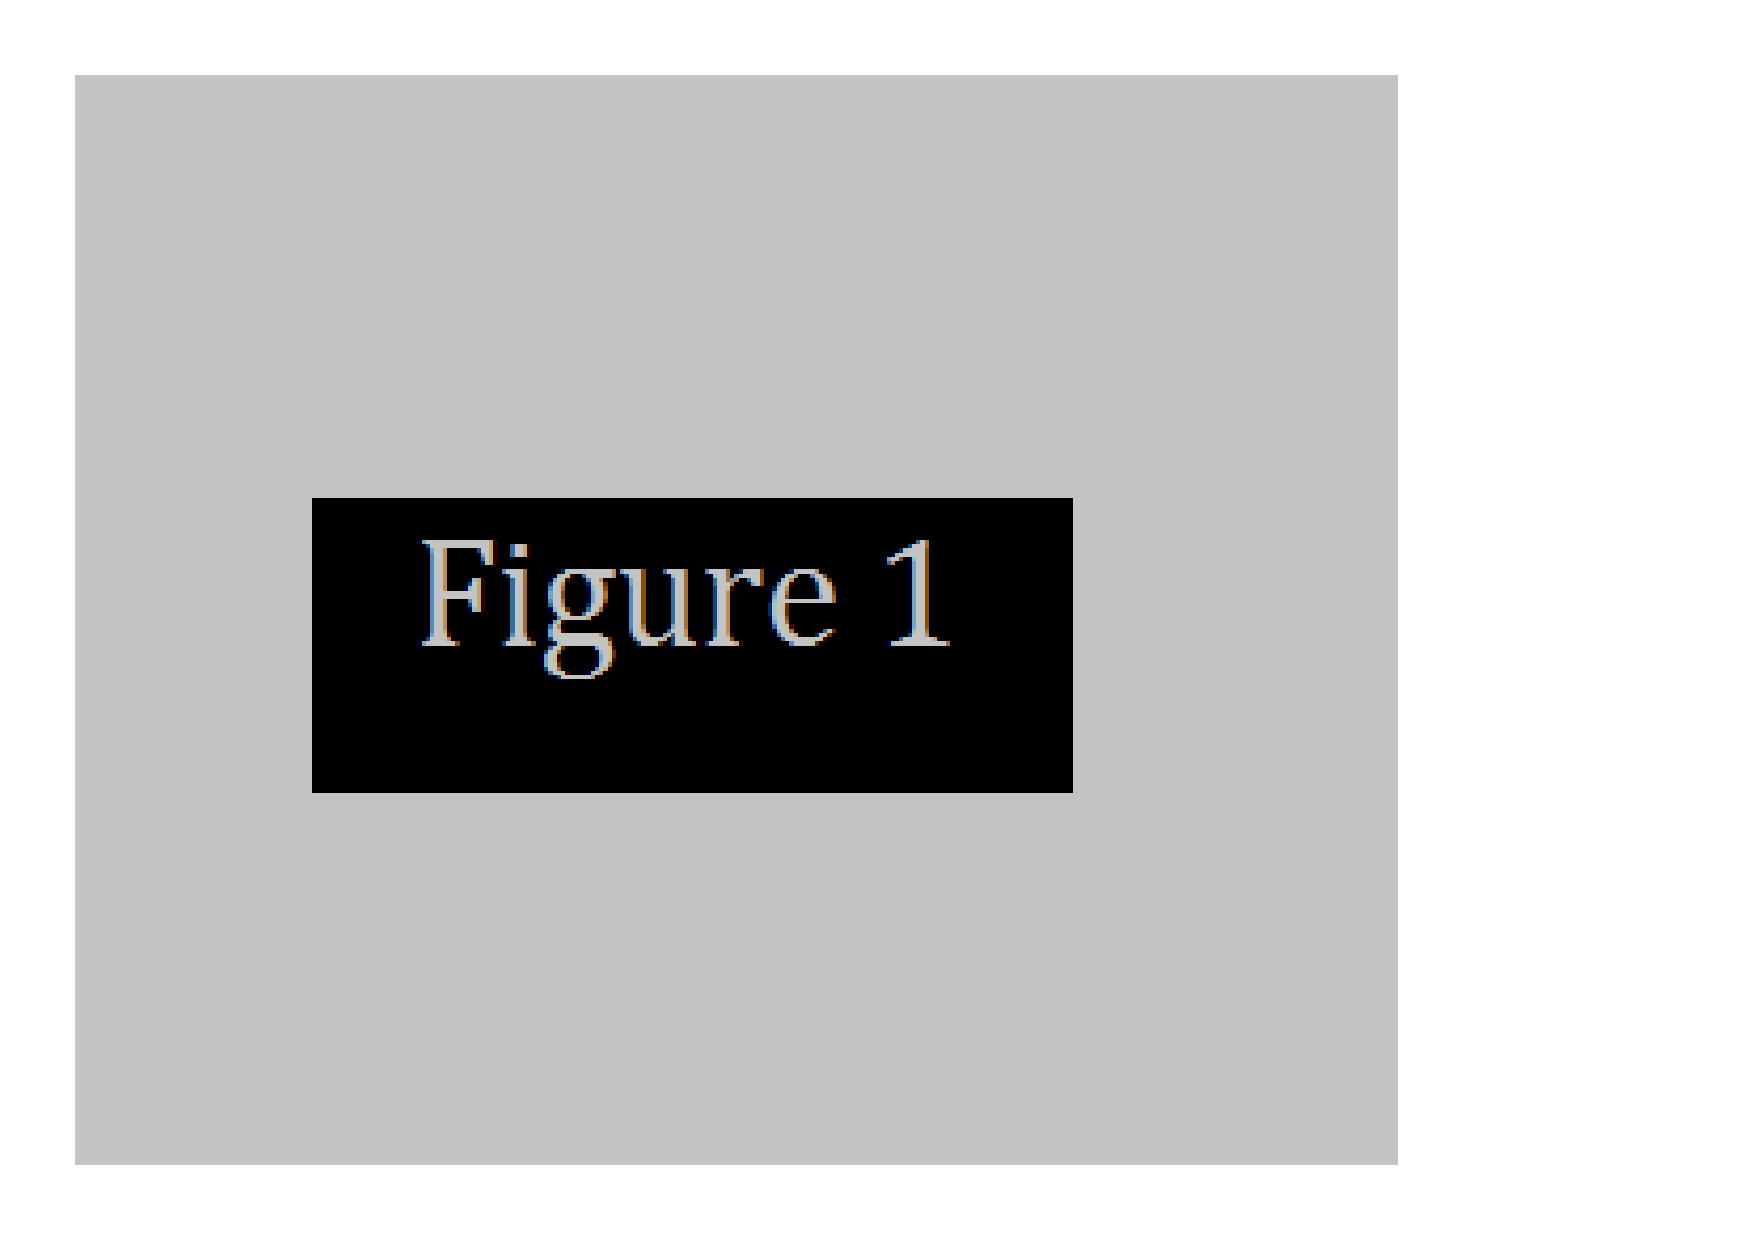
\includegraphics[width=0.2\textwidth]{figure1.pdf}\label{fig:f1}}}}
  \quad % or other spacing between figures
  \subfloat{\makebox[0.4\textwidth]{
\includegraphics[width=0.3\textwidth]{figure2.jpg}\label{fig:f2}}}
  \caption{Multiple images can be inserted inline.}\label{fig:plots}
\end{figure}

\begin{table}[b]
\centering % center-align tables within a column
\caption{This is an example of a single column table. Captions are preferably self-contained and placed above the table. Columns may be left-, center-, decimal marker-, or right-aligned.}\label{table:label1}
\begin{tabular}{l c d{2.3} r}
\toprule
Example & Count 	1			& \multicolumn{1}{c}{Count 2} & Total\\
\midrule
A 						& 2.345 					& 5.435 																		& 16.78(3)\\
B 						& 3.0 							& 12.0																				& 43.2(5)\\
\bottomrule
\end{tabular}
\end{table}

\section{Methodology}

\section{Results and Discussion}

\section{Conclusions}
Here is the Summary or Conclusions section.


\bibliographystyle{spp-bst}
\bibliography{bibfile}

\end{document}